% !TEX root = 99_main.tex

The interest for applying kinetic envelopes in architecture has increased in recent years. On one hand, there is the availability of digital design processes, which enables kinetic concepts to come to life. On the other hand, there is the desire to have active building elements to regulate energy flows to create a more sustainable built environment \cite{loonen2013climate}. 

When analysing the various energy flows, it is solar radiation that is of particular interest. As seen in Figure \ref{fig:ASFschematic} the mediation of solar radiation has the potential to reduce heating and cooling demands, while simultaneously distributing daylight according to the occupants' desires \cite{nagy2016adaptive}. Furthermore, utilising thin film photovoltaic panels as the kinetic element enables the facade to also act as an electricity generator. In Chapter \ref{ch:asfSimulation} I show that such technologies can, in some cases, offset the entire energy consumption of the building space behind the envelope \cite{jayathissa2017optimising}. \\

The application of kinetic architectural envelopes has so far been centred around iconic examples. These include the Al Bahr Towers in Dubai \cite{oborn2012bahr}, the Arab World Institute in Paris, and the ThyssenKrupp Headquarters in Essen. Bringing these technologies to the mainstream, however, can be challenging. 

One major challenge in the design of Kinetic Architectural Elements is the involvement of multiple technological branches. Among these branches we can count structural and energy engineering, control, industrial design, and architecture. Each of these branches has strong interdependencies to each other. For example, during the detail design process, a small variation in the control system such as the range of movement can affect energetic performance and architectural image. This may result in a redesign, that then needs to undergo structural evaluations and fit within the budget. These iteration cycles become a time intensive process that, in some cases, can take months to solve. In order to unite these branches efficiently, new design methods and environments have to be developed. \\

The state of the art in interdisciplinary building design lies in building information modelling (BIM) \cite{schlueter2009building, volk2014building}. The utilisation of BIM to perform fast energy and structural assessments can coordinate the design from its early stages. However, design using BIM is often based on high levels of standardisation, which makes it complicated when designing custom innovative components. The development of kinetic architectural envelopes requires a flexible infrastructure, which allows for fast design, prototyping and production, while maintaining the ability to be customized for each system individually. 

Performative design environments can overcome the limitations of BIM \cite{oxman2008performance}. Performative design takes computer aided design (CAD) in a reversed manner, where it is the simulations that drive the design. Here, the concept of form making, is replaced with form finding. An example of performative design has been described by Turrin et al. where passive solar strategies were explored to improve the thermal comfort and daylight quality under a tessellated roof \cite{turrin2012performative}. This can also stretch to structural performative design in tools such as RhinoVault where the final form is determined through iterative structural simulations \cite{Rippmann2012}. Holzer on the other hand used performative design for direct structural feedback using first and second order structural simulations \cite{holzer2016design}. These tools can also be utilised on the component level, and have been previously analysed in a design studio for smart building envelopes \cite{kim2017exploratory}. However, integrating multiple tools in a single automated environment has still proven to be difficult due to some tools lacking parametrisation capabilities, low openness of the tools interfaces, and low flexibility \cite{diaz2017multidisciplinary,negendahl2015building}. Furthermore, this lack of interoperability results in long iteration cycles, making it difficult to evaluate the necessary trade-offs.\\

This chapter builds on existing knowledge to produce a state of the art performative design environment (PDE) that can shape the form of a facade, provide feedback on its structural strength, analyse the energetic performance and day-lighting conditions of the building space, render images, and produce fabrication drawings for a rapid iterative design process. This is accomplished within the Rhino/Grasshopper environment with python as a scripting language. The methodology is applied in the context of the Adaptive Solar Facade (ASF), a kinetic photovoltaic facade constructed for a research and innovation unit known as the HiLo \cite{Block2017}. HiLo is a two bedroom apartment with a portfolio of energy saving technologies that create a net zero energy building \cite{lydon2017coupling}. Both bedrooms of the HiLo will be equipped with an ASF as seen in Figure \ref{fig:HiLo}. The adaptive control of solar radiation into the bedrooms, coupled with on site electricity generation will contribute to this overall net zero energy strategy.  The entire design process from conceptual design, to prototyping, and final fabrication will be presented.  



The remainder of the chapter is organised as follows: the next section details the parametric design environment and the simulations that drive the final design. Section \ref{ch:results1} describes the outcomes of this design process including the details of the kinetic facade, and Section \ref{ch:conclusion1} discusses the limitations of this environment and concludes the chapter. 



\begin{figure}
\begin{center}
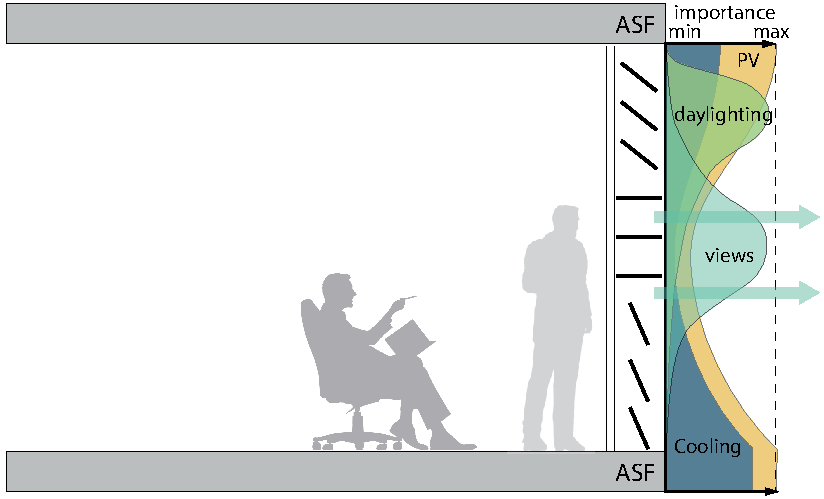
\includegraphics[width=8cm, trim= 0cm 0cm 0cm 0cm,clip]{facadeFunctionsnew.pdf}
\caption{The facade acting as a mediator between the interior and exterior environment, while fulfilling various functions \cite{nagy2016adaptive}}
\label{fig:ASFschematic}
\end{center}
\end{figure}

\begin{figure}
\begin{center}
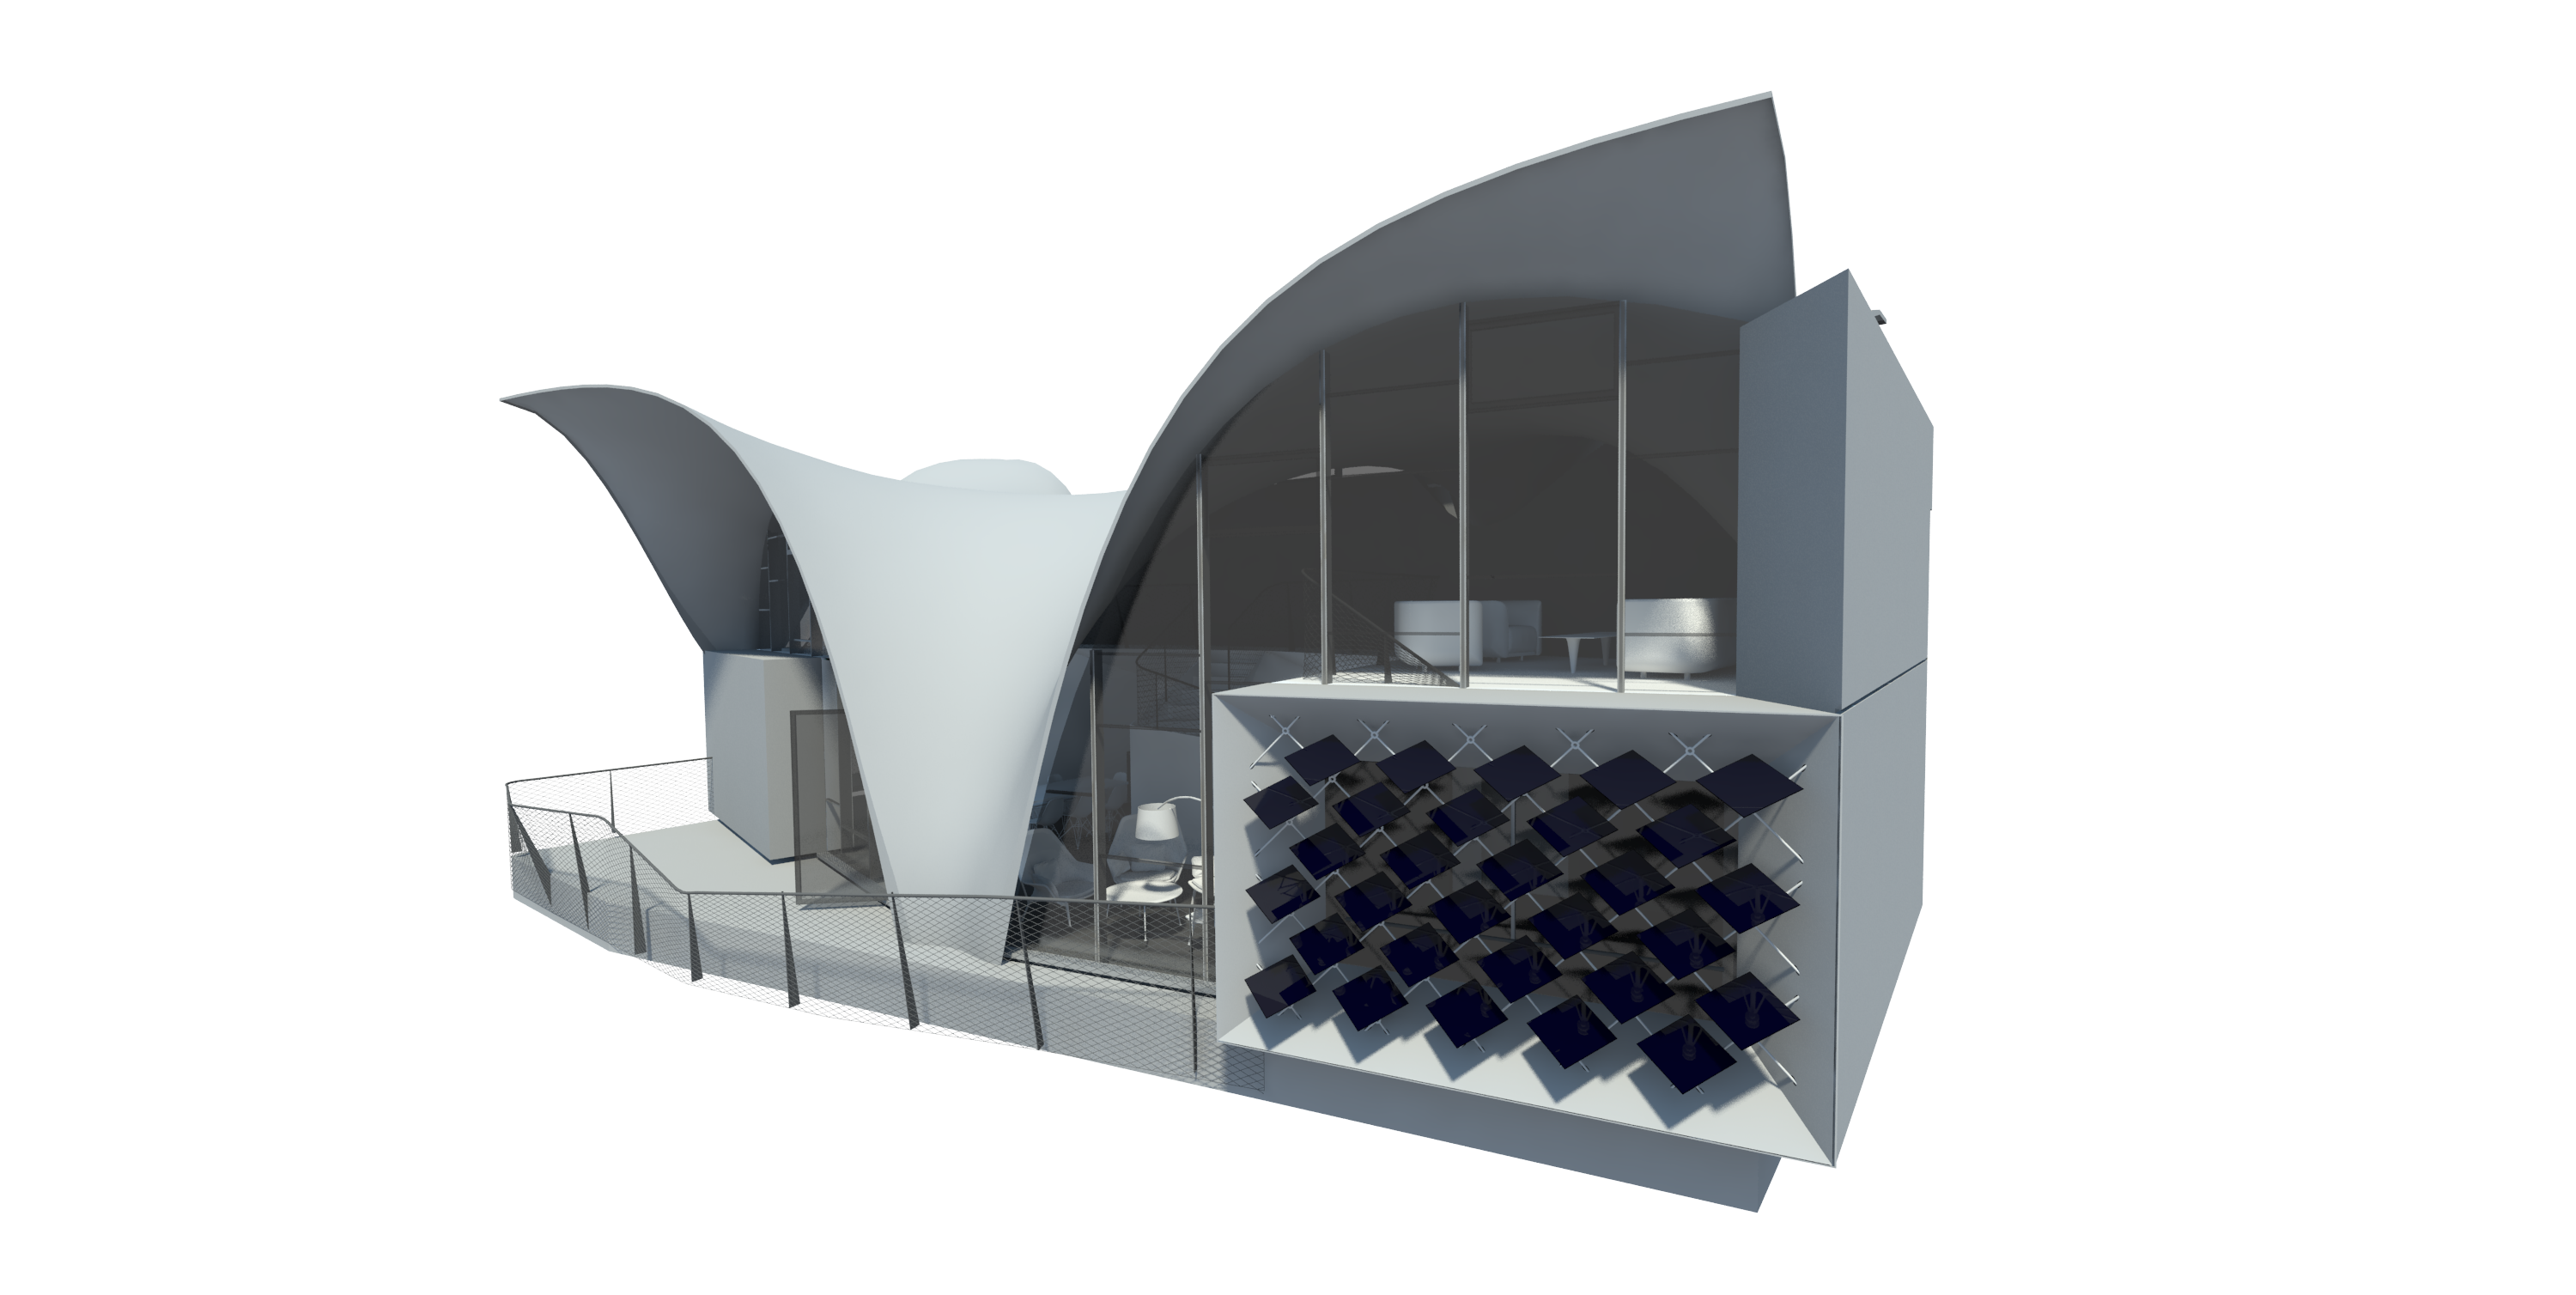
\includegraphics[width=\columnwidth, trim= 0cm 0cm 0cm 0cm,clip]{170719_HiLo_Render_01.png}
\caption{Render of the HiLo module to be constructed in Dubendorf, Switzerland. Two adaptive solar facades have been planned on the south and west facing facades.}
\label{fig:HiLo}
\end{center}
\end{figure}

% \begin{figure}
% \begin{center}
% \includegraphics[width=8cm, trim= 0cm 0cm 0cm 0cm,clip]{honr.jpg}
% \caption{An example of an ASF constructed at the House of Natural Resources \cite{nagy2016adaptive}}
% \label{fig:HoNR}
% \end{center}
% \end{figure}




